\newcommand{\entree}{poids de la lisse $P$}
\newcommand{\delentree}{du \entree}
\newcommand{\lentree}{le \entree}
\newcommand{\sortie}{couple moteur $C_m$}
\newcommand{\delasortie}{du \sortie}
\newcommand{\lasortie}{le \entree}
\newcommand{\correction}{
\begin{center}
 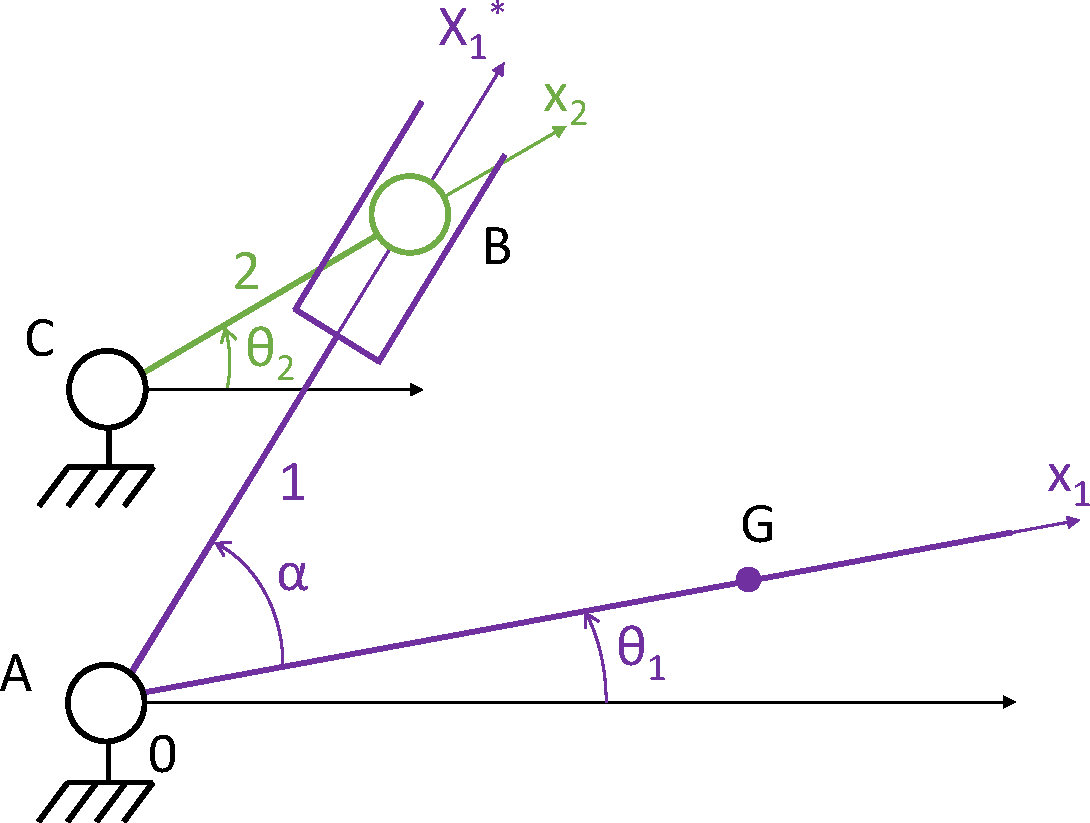
\includegraphics[width=0.6\linewidth]{img/Barriere_cin}
\end{center}

$\left\{T_{P\rightarrow 1}\right\}=\left\{\begin{array}{cc}
0 & \sim \\
-P & \sim \\
\sim & 0
\end{array}\right\}_G=
\left\{\begin{array}{cc}
0 & \sim \\
-P & \sim \\
\sim & (l.cos(\alpha+\theta_1)-L.cos\theta_1).P
\end{array}\right\}_B$

$\left\{T_{C_m\rightarrow 2}\right\}=\left\{\begin{array}{cc}
0 & \sim \\
0 & \sim \\
\sim & C_m
\end{array}\right\}_C=
\left\{\begin{array}{cc}
0 & \sim \\
0 & \sim \\
\sim & C_m
\end{array}\right\}_B$

$\left\{T_{0\rightarrow 1}\right\}=\left\{\begin{array}{cc}
X_{01} & \sim \\
Y_{01} & \sim \\
\sim & 0
\end{array}\right\}_A=
\left\{\begin{array}{cc}
X_{01} & \sim \\
Y_{01} & \sim \\
\sim & -l.cos(\alpha+\theta_1).Y_{01}+l.sin(\alpha+\theta_1).X_{01}
\end{array}\right\}_B$

$\left\{T_{0\rightarrow 2}\right\}=\left\{\begin{array}{cc}
X_{02} & \sim \\
Y_{02} & \sim \\
\sim & 0
\end{array}\right\}_C=
\left\{\begin{array}{cc}
X_{02} & \sim \\
Y_{02} & \sim \\
\sim & -R.cos(\theta_2).Y_{02}+R.sin(\theta_2).X_{02}
\end{array}\right\}_B$

$\left\{T_{2\rightarrow 1}\right\}=\left\{\begin{array}{cc}
0 & \sim \\
Y_{21} & \sim \\
\sim & 0
\end{array}\right\}_{B,R_1^*}=
\left\{\begin{array}{cc}
-sin(\alpha+\theta_1).Y_{21} & \sim \\
cos(\alpha+\theta_1).Y_{21} & \sim \\
\sim & 0
\end{array}\right\}_{B,R_0}$

Isoler 1

$\left\{\begin{array}{l}
X_{01}-sin(\alpha+\theta_1).Y_{21}=0 \\
-P+Y_{01}+cos(\alpha+\theta_1).Y_{21}=0 \\
(l.cos(\alpha+\theta_1)-L.cos\theta_1).P-l.cos(\alpha+\theta_1).Y_{01}+l.sin(\alpha+\theta_1).X_{01}=0
\end{array}\right.$

Isoler 2

$\left\{\begin{array}{l}
X_{02}+sin(\alpha+\theta_1).Y_{21}=0 \\
Y_{02}-cos(\alpha+\theta_1).Y_{21}=0 \\
C_m-R.cos\theta_2.Y_{02}+R.sin\theta_2.X_{02}=0
\end{array}\right.$

Donc, $Y_{21}=\frac{C_m}{R.cos(\theta_1-\theta_2+\alpha)}$

$(l.cos(\alpha+\theta_1)-L.cos\theta_1).P-l.cos(\alpha+\theta_1).(P-cos(\alpha+\theta_1).Y_{21})+l.sin(\alpha+\theta_1).sin(\alpha+\theta_1).Y_{21}=0$

$\frac{L}{l}.P.cos\theta_1=\frac{C_m}{R.cos(\theta_1-\theta_2+\alpha)}$

Donc $C_m=R.cos(\theta_1-\theta_2+\alpha).\frac{L}{l}.P.cos\theta_1$
}

